%% vertical_self_org.tex
In this thesis, two different concepts of self-organisation are implemented.
This chapter presents a method based on vertical self-organisation (c.f. \secref{neuro_concepts_self_org}).
Vertical self-organisation is based on training small units within a network independent from each other.
The first section presents the methodology (i.e. how vertical self-organisation was implemented), and the second section evaluates the obtained results.


\section{Methods}\seclbl{vertical_self_org_methods}
The first choice for networks based on vertical self-organisation is what the independent units are, i.e. which network parameters are trained independently.
In this thesis, a single layer is used as a self-contained unit. One layer is a small unit (e.g. compared to a model part that contains many layers) but can still be trained efficiently.
Smaller units would be neurons or parts of a layer, but training them separately would be very inefficient since the efficiency of matrix operations on GPUs could no longer be fully exploited\sidenote{the layer output can be efficiently calculated by single matrix multiplication and addition, i.e. $\boldsymbol{z} = \boldsymbol{w} \cdot \boldsymbol{x} + \boldsymbol{b}$ (c.f. \secref{ann})}.

Each layer optimises a proxy objective function.
Proxy objective functions are used because this type of local optimisation allows excellent performance even on larger datasets, in contrast to other local learning algorithms such as target propagation, synthetic gradients or feedback alignment (c.f. \secref{alt_train_algo}). 
 \figref{vertical_gradient_flow} visualises the updates based on a proxy objective function.
An objective function is calculated for each layer, and the optimisation algorithm only updates the parameters within this layer.
Thus, the gradients do not flow back to preceding layers.

\begin{figure}[h]
    \centering
    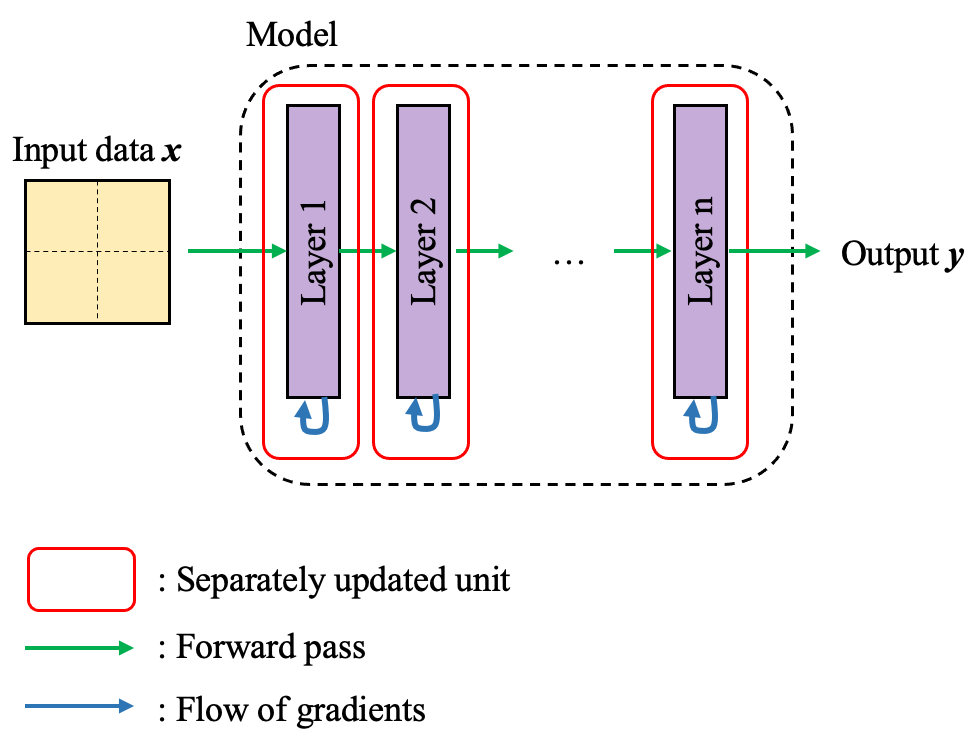
\includegraphics[width=0.99\textwidth]{vertical_gradient_flow}
    \caption[The flow of gradients within the network based on vertical self-organisation]{The flow of gradients within the network based on vertical self-organisation: The data is fed from layer to layer during the forward pass. The layers are trained independently, and the gradients do not flow from one layer to the previous one.}
    \figlbl{vertical_gradient_flow}
\end{figure}

A combination of diversity and sparsity constraints is used as a loss function, which leads to representations that are easy to interpret, suitable for net fragments (c.f. \secref{neuro_concepts_net_fragments}), and also increases robustness (c.f. \secref{neuro_concepts_sparsity}).
Identical to the preliminary experiments in appendix \chref{net_fragments}, the sparsity is achieved by using the kullback-leibler (KL) divergence \sidecite{10-5555-3042573-3042641}.
The model consists of several linear layers $l$ with a ReLU activation function (c.f. \eqref{act_functions}).

A layer consists of $n^{[l]}$ neurons and the activations $\boldsymbol{a}^{[l]}$ of a linear layer $l$ are calculated for a given input $\boldsymbol{a}^{[l-1]}$ as

\begin{align}\eqlbl{vso_1}
		\boldsymbol{a}^{[l]} = a^{[l]}_1, ..., a^{[l]}_n = \boldsymbol{W}^{[l]} \cdot \boldsymbol{a}^{([l-1]} + \boldsymbol{b}^{[l]}
\end{align}

whereby $\boldsymbol{W}^{[l]}$ is the weight and $\boldsymbol{b}^{[l]}$ the bias of layer $l$.
The activation probability can be calculated for each neuron. If a mini-batch contains $m$ samples, the activation probability $\hat{\rho}^{[l]}_i$ of a neuron $a^{([l]}_i$ can be calculated as:

\begin{align}\eqlbl{vso_2}
		\hat{\rho}^{[l]}_i= \frac{1}{n} \sum^n_{i=1} \left( \frac{1}{1+e^{-a^{([l]}_i}} \right)
\end{align}

where $\left( \frac{1}{1+e^{-a^{([l]}_i}} \right)$ is the sigmoid function that squeezes the activation in the range between $0$ and $1$.
With the KL divergence, the divergence of the current activation probability $\hat{\rho}^{[l]}_i$ and a desired activation probability $\rho=0.05$ can be calculated:

\begin{align}\eqlbl{vso_3}
		KL(\rho || \hat{\rho}^{[l]}_i) = \rho \cdot \log \frac{\rho}{\hat{\rho}^{[l]}_i} + (1-\rho) \cdot \log \frac{1-\rho}{1-\hat{\rho}^{[l]}_i}
\end{align}

The sparsity loss $\mathcal{L}^{[l]}_{s}$ of layer $l$ is the sum of the divergence between all $\hat{\rho}^{[l]}_i$ and $\rho$:

\begin{align}\eqlbl{vso_4}
		\mathcal{L}^{[l]}_{s}(\rho, \hat{\rho}^{[l]}) = \sum_{i=1}^{m} KL(\rho || \hat{\rho}^{[l]}_i)
\end{align}


The second constraint is a diversity constraint. The goal is that the activations of \emph{different} objects are diverse. For this purpose, the activations $\boldsymbol{a}^{[l]}$ are made as identical as possible (i.e. pushed together in feature space) if they stem from the same class and as different as possible if they stem from different classes.
The cosine similarity is used to calculate the similarity between the activations $\boldsymbol{a}^{[l](i)}$ and $\boldsymbol{a}^{[l](j)}$ of two samples $\boldsymbol{x}^{(i)}$ and $\boldsymbol{x}^{(j)}$:

\begin{align}\eqlbl{vso_5}
		\text{cos}\left( \boldsymbol{a}^{[l](i)}, \boldsymbol{a}^{[l](j)} \right) = \frac{\boldsymbol{a}^{[l](i)} \cdot \boldsymbol{a}^{[l](j)}}{\max \left( ||\boldsymbol{a}^{[l](i)}||_2, ||\boldsymbol{a}^{[l](j)}||_2 \right)}
\end{align}

The information of image labels $y^{(i)} \in C$ is needed to push representations of identical objects together or to push representations of different objects apart.
The diversity loss $\mathcal{L}^{[l]}_d$ minimises the similarity $\text{cos} \left(\boldsymbol{a}^{[l](i)}, \boldsymbol{a}^{[l](j)} \right)$ if the activations stem from different classes (i.e. $y^{(i)} \neq y^{(j)}$), or maximises the similarity if they stem from the same class (i.e. $y^{(i)} = y^{(j)}$).

\begin{align}\eqlbl{vso_6}
		\mathcal{L}^{[l]}_{d} \left(\boldsymbol{a}^{[l]} \right) = \frac{1}{n^2} \sum_{i=1}^{n} \sum_{j=1}^{n} k \cdot \text{cos} \left( \boldsymbol{a}^{[l](i)}, \boldsymbol{a}^{[l](j)} \right) \text{ if } i \neq j
\end{align}

whereby $k$ changes the sign depending on the class:

\begin{align}\eqlbl{vso_7}
		k = \begin{cases}
      		+1, & \text{if}\ y_i \neq y_j \\
      		-1, & \text{otherwise}
    	\end{cases}
\end{align}

However, the loss was found to be more stable if the similarity is not calculated between two activations but between one activation and the average activation of a class. The average activation $\overline{a[c]}$ of a class $c$ can be calculated over $n_c$ samples as:

\begin{align}\eqlbl{vso_8}
		\overline{a[c]^{[l]}} = \frac{1}{n_c} \sum_{i=1}^{n_c} a^{[l]}_i \text{, for } y_i = c
\end{align}

Thus, the loss becomes
\begin{align}\eqlbl{vso_80}
		\mathcal{L}^{[l]}_{d} \left(\boldsymbol{a}^{[l]} \right) = \frac{1}{n\cdot n_c} \sum_{i=1}^{n} \sum_{c \in C} k \cdot \text{cos} \left( \boldsymbol{a}^{[l](i)}, \overline{\boldsymbol{a}[c]}^{[l]} \right)
\end{align}

Another problem of this loss is that if all activations are identical, then $\text{cos} \left(\boldsymbol{a}^{[l](i)}, \overline{\boldsymbol{a}[c]}^{[l]} \right) = 1$, and the loss becomes $\mathcal{L}^{[l]}_{d}=0$, since the similarities of the same and different classes neutralise each other.
Therefore, a margin between the similarities is enforced, as done for the triplet-margin-loss  \sidecite{Balntas_Riba_Ponsa_Mikolajczyk_2016}.

\begin{align}\eqlbl{vso_9}
\begin{split}
		\mathcal{L}^{[l]}_{d}(\boldsymbol{a}^{[l]}) = \frac{1}{n} \sum_{i=1}^{n} \max \biggl[ & \text{cos}(\boldsymbol{a}^{[l](i)}, \overline{a[v]^{[l]}}) \\
		& - \text{cos}(\boldsymbol{a}^{[l](i)}, \overline{a[y^{(i)}]^{[l]}}) + \text{margin}, 1 \biggr]
\end{split}
\end{align}

where $v$ is a random class drawn from the set $v ~ \{C \\ y_i\}$ and $\text{margin}$ is a hpyer-parameter that was set to $1$.
Thus, the triplet-margin-loss is calculated but the cosine-similarity replaces the $L2$-norm as distance measure and the positive, resp. negative anchor is replaced with the average class activation from the same resp. from a randomly selected different class.

The loss used is the sum of sparsity loss and diversity loss, with the diversity loss weighted by $\lambda=0.1$:
\begin{align}\eqlbl{vso_10}
		\mathcal{L}^{[l]} =\mathcal{L}^{[l]}_{s}(\rho, \hat{\rho}^{[l]}) 
 + \lambda \cdot \mathcal{L}^{[l]}_{d}(\boldsymbol{a}^{[l]})
\end{align}


One problem with proxy objective functions is that this type of training often requires layer-wise training. First, layer $1$ is trained until convergence, then the weights are frozen, then layer $2$ is trained and so on.
Such sequential training is inefficient because it requires more forward passes than if the model is trained with end-to-end backpropagation.
It was found that this loss function allows to train all layers simultaneously. With a forward pass, all activations are calculated, followed by a layer-wise backward pass where the gradients from one layer do not propagate back into the previous layer.
Since the gradients are only needed locally, no large graph of gradients has to be calculated, which reduces the memory utilisation on GPUs and allows larger mini-batch sizes. In addition, this type of architecture is straightforward to parallelise since each layer (i.e. each independently trained unit) or a group of layers can be trained on a different GPU:
In contrast to end-to-end backpropagation of error architectures, the gradients only flow backwards locally on a GPU and do not have to be passed on to other GPUs.

\begin{figure}[h]
    \centering
    \resizebox{0.99\textwidth}{!}
{
\begin{tikzpicture}
\tikzstyle{connection}=[ultra thick,every node/.style={sloped,allow upside down},draw=\edgecolor,opacity=0.7]
\tikzstyle{copyconnection}=[ultra thick,every node/.style={sloped,allow upside down},draw={rgb:blue,4;red,1;green,1;black,3},opacity=0.7]


\node[canvas is zy plane at x=0] (input) at (0,0,0) {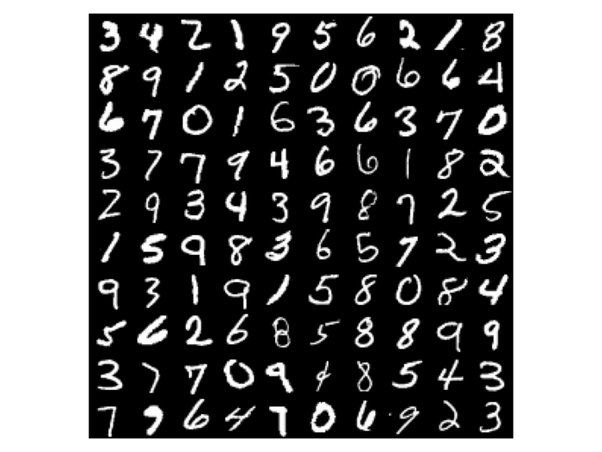
\includegraphics[width=8cm,height=8cm]{imgs/mnist.jpeg}};


\pic[shift={(3,0,0)}] at (input) 
    {Box={
        name=fcn1,
        caption=FC + ReLU,
        xlabel={{" ","dummy"}},
        zlabel=512,
        fill=\SoftmaxColor,
        opacity=0.8,
        height=3,
        width=3,
        depth=52
        }
    };


\draw [connection]  (input) ++(0,0,0)    -- node {\midarrow} (fcn1-west);


\pic[shift={(2,0,0)}] at (fcn1-east) 
    {Box={
        name=fcn2,
        caption=FC + ReLU,
        xlabel={{" ","dummy"}},
        zlabel=256,
        fill=\SoftmaxColor,
        opacity=0.8,
        height=3,
        width=3,
        depth=25
        }
    };


\draw [connection]  (fcn1-east)    -- node {\midarrow} (fcn2-west);


\pic[shift={(2,0,0)}] at (fcn2-east) 
    {Box={
        name=fcn3,
        caption=FC + ReLU,
        xlabel={{" ","dummy"}},
        zlabel=128,
        fill=\SoftmaxColor,
        opacity=0.8,
        height=3,
        width=3,
        depth=13
        }
    };


\draw [connection]  (fcn2-east)    -- node {\midarrow} (fcn3-west);


\pic[shift={(2,0,0)}] at (fcn3-east) 
    {Box={
        name=fcn4,
        caption=FC + ReLU,
        xlabel={{" ","dummy"}},
        zlabel=64,
        fill=\SoftmaxColor,
        opacity=0.8,
        height=3,
        width=3,
        depth=6
        }
    };


\draw [connection]  (fcn3-east)    -- node {\midarrow} (fcn4-west);


\end{tikzpicture}
}
    \caption[Architecture of the fully connected model with vertical self-organisation]{The network architecture of the fully connected model for vertical self-organisation with fully connected layers.}
    \figlbl{vertical_org_arch1}
\end{figure}

The model used consists of $4$ fully connected layers with ReLU activation. The first layer has $512$ neurons, the second $256$ neurons, the third $128$ neurons and the fourth $64$ neurons. The model is illustrated in Figure \figref{vertical_org_arch1}. Each layer is trained separately by minimising the loss of equation \eqref{vso_10} with the Adam optimizer\sidecite{Kingma2015AdamAM} and a learning rate of $\eta = 1 \cdot 10^{-3}$. The mini-batch size is $60,000$. 

\subsection{Extraction of Representations}\seclbl{vertical_self_org_representations}
In accordance with net fragments as in \secref{neuro_concepts_net_fragments}, the representations are not extracted at a specific point in the network (i.e. a pre-defined layer), but all representations from all layers are taken into account to fulfil a task.
In the following, this is demonstrated based on a classification task, but other tasks are also conceivable in the future.
After training, the average activation $\overline{\boldsymbol{a}[c]}^{[l]}
$ for each class $c \in C$ and layer $l$ is determined, as done in Equation \eqref{vso_8}.
These averages from the training set represent prototypes of each class in each layer and can be considered a reference representation per class. Thus, the representations needed for this task are computed \emph{after} training and are not part of the training as, for example, in the case of a classification loss based on cross-entropy.
When a new sample $\boldsymbol{x}^{(i)}$ is classified, the cosine similarity between the activations $\boldsymbol{a}^{[l](i)}$ of this sample and the class prototypes $\overline{\boldsymbol{a}[c]}^{[l]}$ is calculated in each layer.

\begin{align}\eqlbl{vso_11}
		\text{cos}[c]^{[l](i)} = \text{cos} \left( \boldsymbol{a}^{[l](i)}, \overline{\boldsymbol{a}[c]}^{[l]} \right) = \frac{\boldsymbol{a}^{[l](i)} \cdot \overline{\boldsymbol{a}[c]}^{[l]}}{\max \left( ||\boldsymbol{a}^{[l](i)}||_2, ||\overline{\boldsymbol{a}[c]}^{[l]}||_2 \right)} \text{, for } c \in C
\end{align}

Thus, the cosine similarity $\text{cos}[c]^{[l](i)}$ for each class $c \in C$ and each of the layers $l \in {1, ..., 4}$ is calculated. Afterwards, the class $c$ with the highest average cosine similarity between the sample activations $\boldsymbol{a}^{[l](i)}$ and the class prototypes $\overline{\boldsymbol{a}[c]}^{[l]} 
$ is used as prediction.

\begin{align}\eqlbl{vso_12}
		\argmax_{c \in C} \frac{1}{4} \sum_{l=1}^{4} \text{cos}[c]^{[l](i)}
\end{align}

This results in a weighted voting; if a layer is certain that the sample belongs to a specific class, the sample has a high cosine similarity with one class prototype and a low similarity with all other class prototypes. Accordingly, this layer influences the prediction more than a layer that cannot assign the sample to one class and calculates a similarly high cosine similarity between the sample and all prototypes.

\subsection{Lateral Connections}
As described in \secref{neuro_concepts_lateral_connections}, lateral connections in the human brain serve neurons to support each other.
There, it is also described that lateral connections can be implemented as recurrent connections.
There are several ways to implement recurrent connections. A straightforward possibility is to concatenate the layer input $\boldsymbol{a}^{[l-1]}[t]$ at time $t$ with the layer output $\boldsymbol{a}^{[l]}[t-1]$  at time $t-1$. This is visualised in \figref{lateral_concat}. Of course, $\boldsymbol{a}^{[l]}[t-1]$ is undefined at $t=0$. In this case, $\boldsymbol{a}^{[l]}[t-1]$ is initialized with zeros.

\begin{figure}[h]
    \centering
    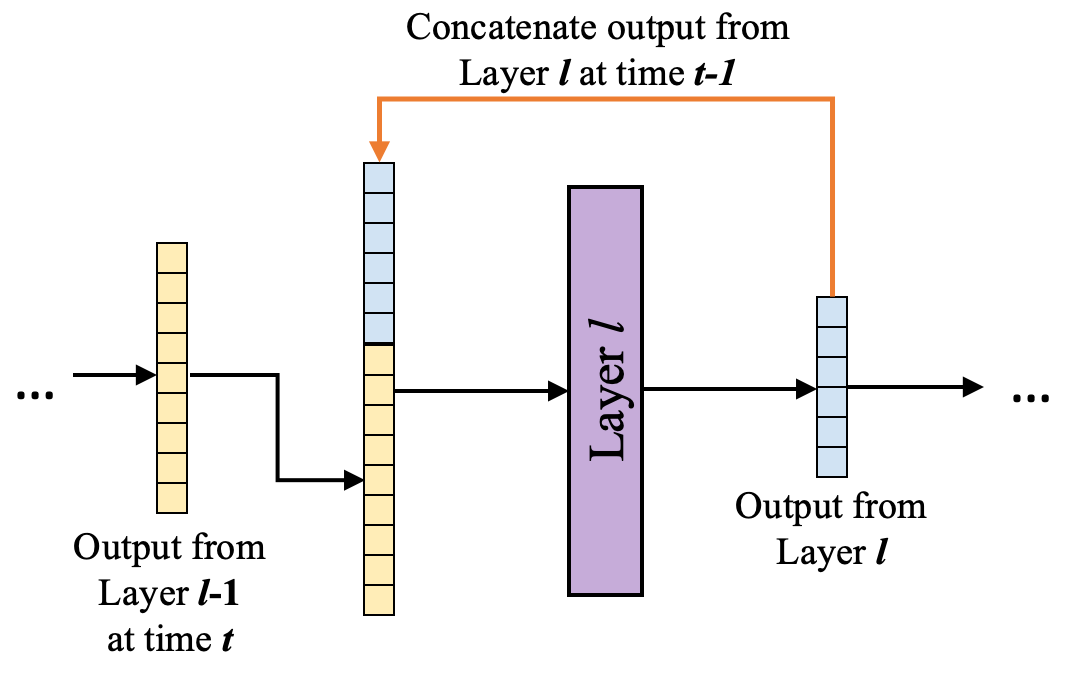
\includegraphics[width=0.99\textwidth]{lateral_concat}
    \caption[Lateral connections by concatenating the layer's output with the layer's input]{The lateral connections can be implemented by concatenating the layer's output at the previous time-step with the layer's input at the current time-step.}
    \figlbl{lateral_concat}
\end{figure}


A second option is to use a second weight matrix, as it is usually done in recurrent layers. Therefore, the equation \eqref{vso_1} is extended as follows:

\begin{align}\eqlbl{vso_13}
		\boldsymbol{a}^{[l]}[t] =  \boldsymbol{W}_x^{[l]} \cdot \boldsymbol{a}^{[l-1]}[t] + \boldsymbol{b}^{[l]} + \overbrace{\boldsymbol{W}_h^{[l]} \cdot \boldsymbol{a}^{[l]}[t-1] }^{\text{lateral connection}}
\end{align}

whereby $\boldsymbol{W}_x^{[l]}$ is the weight multiplied with the layer input and $\boldsymbol{W}_h^{[l]}$ the weight multiplied with the previous layer output. In both cases, the layer receives information about the activations at the previous time step.
However, this only seems helpful if the model input is not static. Therefore, the model input is available over several time steps and is augmented after each step. Thus, the model receives different views of the same image and can adjust its activations from the previous time step if necessary. The following image augmentation techniques are applied, each with a probability of $p=0.8$:

\begin{itemize}
	\item \textbf{Color Jitter}: Randomly change brightness, contrast, and saturation of the image.
	\item \textbf{Gaussian Blur}: Blur the image with randomly chosen Gaussian blur.
	\item \textbf{Random Rotation}: Randomly rotate the image with an angle in the range $[-15°, ..., 15°]$
	\item \textbf{Adjust Sharpness}: Randomly adjust the sharpness of the image.
\end{itemize}

\figref{mnist_augmented} visualises how this augmentation affects samples of the MNIST dataset \cite{Lecun_Bottou_Bengio_Haffner_1998}. The original image is shown on the left, and $9$ augmented versions of it are shown on the right. This allows the model to perceive the same image from different views.

\begin{figure}[h]
    \centering
    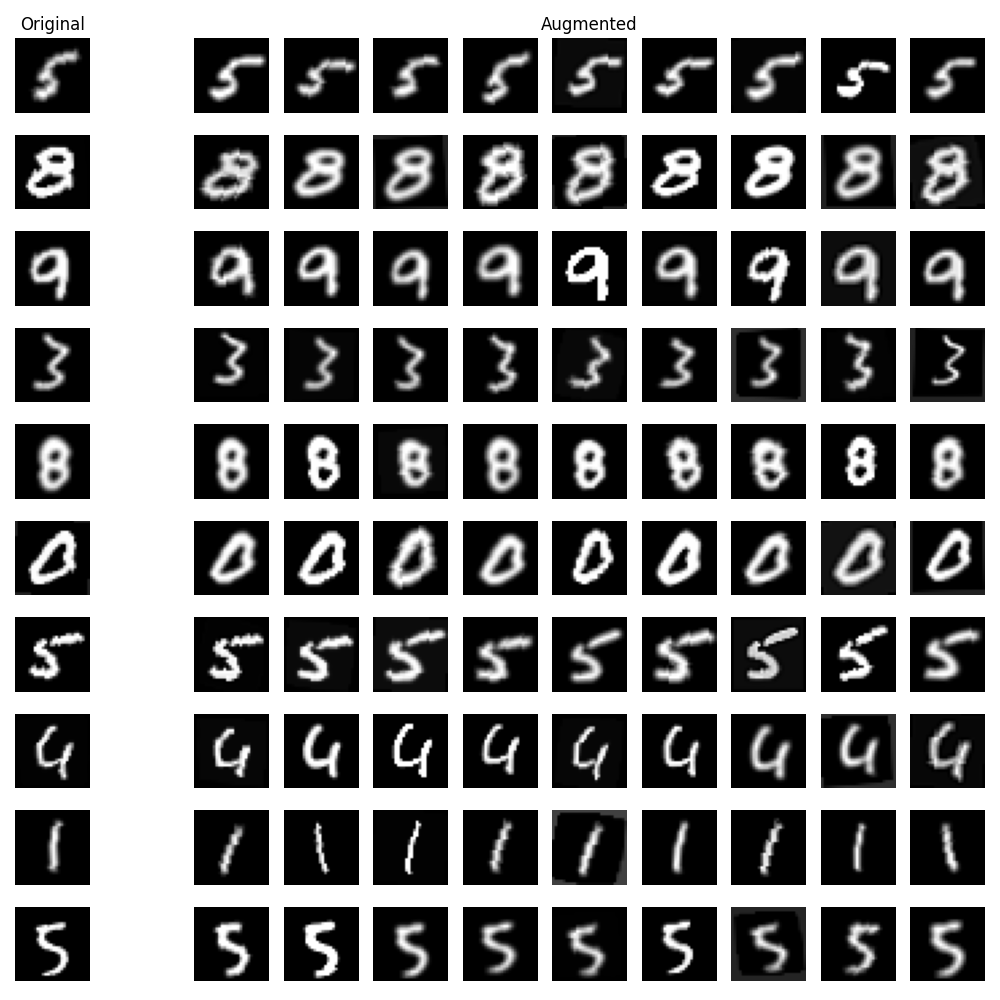
\includegraphics[width=0.99\textwidth]{mnist_augmented}
    \caption[Data augmentation applied on $10$ samples of the MNIST dataset]{Data augmentation applied on $10$ samples of the MNIST dataset. The original samples from the dataset are shown on the left, and $9$ augmented versions of the same samples are shown on the right.}
    \figlbl{mnist_augmented}
\end{figure}


Recurrent connections, which in this context represent lateral connections, are typically used to process sequential data or text. In this case, the data is collected cumulatively before an output is generated. For example, in text processing, all word tokens of a sentence are typically read before the model classifies a sentence. This is necessary because all information is required, and classification cannot be done on the basis of a single token. Such models are typically trained with backpropagation through time (BTT). Thereby, the gradients flow backwards over several time steps. This leads to well-known problems such as vanishing and exploding gradients.

In this thesis, BTT is not used, which means that a prediction is made after each time step, but the prediction potentially improves with more time steps. This leads to desirable properties: (i) Problems with vanishing or exploding gradients do not exist, regardless of how many time steps the model requires. (ii) After each time step, representations can be extracted according to \secref{vertical_self_org_representations}. If an object representation can be assigned to one class label with a high probability, the sequential processing of different image views can be aborted. If this is not the case, further time steps can be carried out until the model has sufficiently high confidence in its prediction. Thus, the number of time steps can be sample-dependent.


% Idee: Mehr Robustheit indem z.b. in einem timestep noise als Input genutzt wird oder bei 1 von 10 timesteps (ausser in den ersten 2) das Bild zufälligerweise vertauscht wird. -> Lateral connections should help

\subsection{Hierarchical Features}\seclbl{vertical_self_org_hierarchical_features}
A criticism of the proposed model is that it does not learn hierarchical features, even though hierarchical features are one of the main reasons for the excellent performance of deep learning systems. The diversity loss (c.f. \eqref{vso_9})  enforces in each layer that the latent representations of objects of the same class are similar and that the representations of different classes are different. This violates the concept of hierarchical features; the first layers should learn general features that are helpful for all classes but cannot necessarily be assigned to a specific class. Only later layers build class representations that are specific to a class. In the current setting, however, already the first layers generate class-specific representations.

In the following, three possible measures are described to counteract this problem: (i) The fully connected layers are replaced by convolutional layers so that the first layers have a smaller field of view and can only recognise local features. (ii) An adapted version of the diversity loss enforces a separation of features by class only in the last layers. (iii) While specific information in the form of the input image flows into the network from one side, general information in the form of class labels is fed into the network from the other side, and these two types of information are fused. Thus, the training process enforces a hierarchy by fusing specific and general information over multiple layers.
These three measures can be applied either individually or in combination with each other.


\subsubsection{Convolutional Architecture}
In a CNN, the field of view in the first layers is restricted by design but becomes larger in subsequent layers. Consequently, using a CNN architecture instead of a model based on fully connected layers alleviates the problem of non-hierarchical features.


\begin{figure}[h]
    \centering
    \resizebox{0.99\textwidth}{!}
{
\begin{tikzpicture}
\tikzstyle{connection}=[ultra thick,every node/.style={sloped,allow upside down},draw=\edgecolor,opacity=0.7]
\tikzstyle{copyconnection}=[ultra thick,every node/.style={sloped,allow upside down},draw={rgb:blue,4;red,1;green,1;black,3},opacity=0.7]


\node[canvas is zy plane at x=0] (input) at (0,0,0) {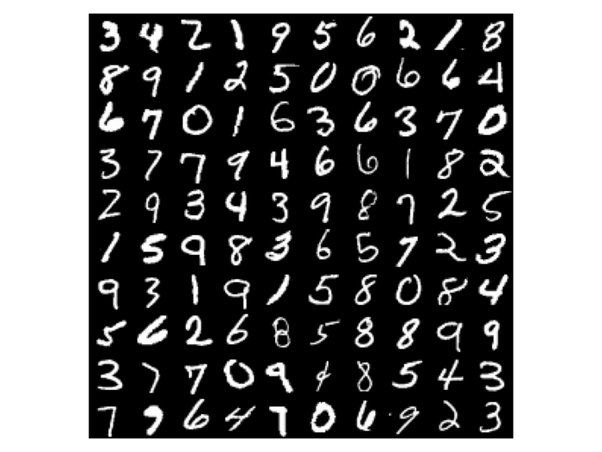
\includegraphics[width=8cm,height=8cm]{imgs/mnist.jpeg}};


\pic[shift={(3,0,0)}] at (input) 
    {Box={
        name=conv1,
        caption=Conv + ReLU,
        xlabel={{1, }},
        zlabel=16,
        fill=\ConvColor,
        height=16,
        width=2,
        depth=16
        }
    };


\draw [connection]  (input) ++(0,0,0)    -- node {\midarrow} (conv1-west);


\pic[shift={ (0,0,0) }] at (conv1-east) 
    {Box={
        name=pool1,
        caption= ,
        fill=\PoolColor,
        opacity=0.5,
        height=8,
        width=1,
        depth=8
        }
    };


\pic[shift={(2,0,0)}] at (pool1-east) 
    {Box={
        name=conv2,
        caption=Conv + ReLU,
        xlabel={{16, }},
        zlabel=32,
        fill=\ConvColor,
        height=8,
        width=4,
        depth=8
        }
    };


\draw [connection]  (pool1-east)    -- node {\midarrow} (conv2-west);


\pic[shift={ (0,0,0) }] at (conv2-east) 
    {Box={
        name=pool2,
        caption= ,
        fill=\PoolColor,
        opacity=0.5,
        height=4,
        width=1,
        depth=4
        }
    };


\pic[shift={(2,0,0)}] at (pool2-east) 
    {Box={
        name=conv3,
        caption=Conv + ReLU,
        xlabel={{32, }},
        zlabel=64,
        fill=\ConvColor,
        height=4,
        width=6,
        depth=4
        }
    };


\draw [connection]  (pool2-east)    -- node {\midarrow} (conv3-west);


\end{tikzpicture}
}
    \caption[Architecture of the CNN for vertical self-organisation]{The network architecture of the CNN for vertical self-organisation with fully connected layers.}
    \figlbl{vertical_org_arch2}
\end{figure}

The CNN architecture used in this thesis is shown in \figref{vertical_org_arch2}.
Three convolutional layers with ReLU activation functions and with $16$, $32$, and $64$ channels are used, and max-pooling layers are applied between each convolutional layer. For training, the same hyperparameters and loss functions are used as for the model with fully connected layers.

\subsubsection{Hierarchical Diversity Loss}
A second measure to obtain hierarchical features is to adapt the diversity constraint of the loss function. The current version forces the latent representations of objects of the same class to be similar and those of different classes to be different. This is useful in the last layers, where high-level features (i.e. high-level net fragments) or object representations should be detected and separated from each other. In the first layers, on the other hand, the separation should not depend on the class label. Nevertheless, the activations should also be diverse if low-level features are detected (c.f. Section \secref{neuro_concepts_net_fragments}).

Therefore, the sparsity constraint is split into two parts: One part ensures that the activations within a (large) mini-batch are diverse and thus enforces that different features are captured and represented by different neurons. The second part ensures, as before, that the activations are diverse for different classes. Thus, one part of the constraint ensures \emph{diversity within the mini-batch} and the other part ensures \emph{diversity between different classes}.

These two parts are weighted linearly from the first to the last layer. Since the first layer should have a high diversity within the mini-batch, it has a high weight on the first part of the diversity constraint and a low weight on the second part. The last layer has an inverse weighting and pays more attention to the diversity constraint's second part than the first part.

The first part of the diversity constraints ensures diversity within a mini-batch. This is achieved by ensuring that each neuron within a mini-batch should be active. 

TODO: At the moment, various experiments are still ongoing to find out how this can be implemented (therefore, not yet explained in more detail).


\subsubsection{Two-Way Information Flow}
Hinton \sidecite{ff_algo} introduced with the forward-forward (FF) algorithm (c.f. Section \secref{alt_train_algo}) a promising idea for models based on proxy objective functions: 
The image is fed into the input layer of the network, and the corresponding label is fed into the output layer of the network. The image remains static for several time steps, and the network is trained to push the layer's activations above a certain threshold. In a second stage, the image is fed into the network with the wrong label and the network is trained to push the activations below a certain threshold. He found that a feature hierarchy is created when low-level features (i.e. images) are fed into the network from one end and high-level features (i.e. class labels) are fed into the network from the other end. However, this approach has one major disadvantage: During inference, each possible sample-label combination has to be fed into the model, and the label that caused the highest neural activity is used as the model's prediction.

In this thesis, this is implemented in a different way, which does not have this disadvantage. Identical to the FF algorithm, the image is fed into the network's input layer for multiple time steps. Conversely, the label is not fed directly into the output layer but is made available to the last layer within the loss function. Each layer maximises the mutual information (MI) between its activations and the activations of the previous and subsequent layers. Thus, the first layer maximises the MI between the input image and its activations, the last layer maximises the MI between its activations and a label vector. This creates a feature pyramid in which a smooth transition from concrete samples to abstract class labels is learned. During inference, the last layer directly predicts latent representations that can be assigned to a class.

\begin{figure}[h]
    \centering
    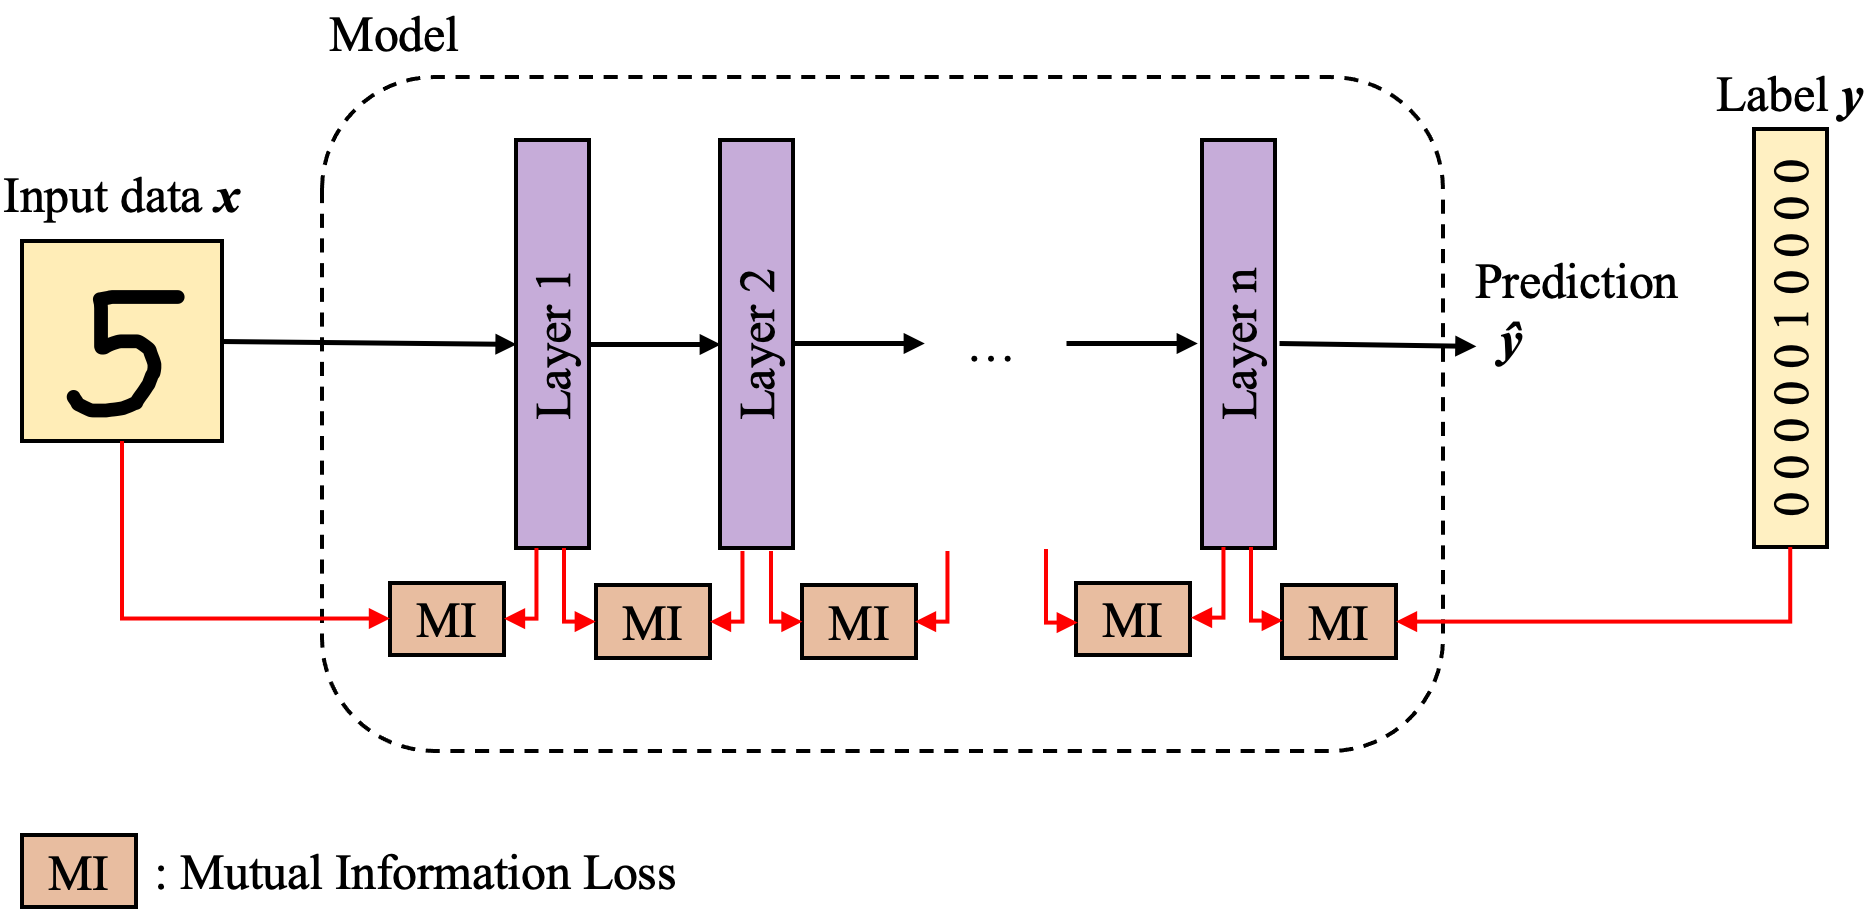
\includegraphics[width=0.99\textwidth]{mi_loss}
    \caption[Vertical self-organisation with mutual information loss]{Vertical self-organisation with mutual information loss: Each layer maximises the mutual information (MI) between its activations and the activations of the previous and subsequent layers. The first layer maximises the MI between its activations and the input image (instead of the previous layer), and the last layer maximises the MI between its activations and the image label (instead of the subsequent layer).}
    \figlbl{mi_loss}
\end{figure}

This process is visualised in Figure \figref{mi_loss}. 


TODO: Currently, various experiments are ongoing to find out how this can be implemented (therefore, yet to be explained in more detail).


%\subsection{Efficient Parallel Training}
%Idee: Nachfolgelayer einbeziehen in Loss -> Nachfolgelayer ist gefroren, Output muss aber möglichst gut sein (sollte Performance nicht verschlechtern von Nachfolgelayer) + eigene Performance verbessern


\section{Results}\seclbl{vertical_self_org_methods_results}
The results obtained by this model are presented below. It is important to note that these models aim not to achieve the best possible results in terms of classification accuracy on a benchmark. In large-scale comparisons, it has often been found that end-to-end backpropagation of error is far superior to other methods, especially in image classification \sidecite{Bartunov_Santoro_Richards_Marris_Hinton_Lillicrap_2018}. Instead, the aim here is to examine interesting concepts that are more biologically plausible and can inspire future work.

\subsection{Dataset}\seclbl{vertical_self_org_methods_dataset}
The model was trained and evaluated on the MNIST \cite{Lecun_Bottou_Bengio_Haffner_1998} dataset. It is a dataset of handwritten digits with $60'000$ training samples and $10'000$ test samples.
In this thesis, the predefined training and test split is used.
The samples are images of a digit with the resolution $28 \times 28$ pixel in grayscale, i.e. has one colour channel.

In addition, the models are evaluated on MNIST-C \sidecite{Mu_Gilmer_2019}, a corrupted MNIST benchmark for testing the out-of-distribution robustness of image classification models. This dataset consists of the MNIST data with $15$ types of corruptions applied to the samples.

\subsection{Baseline Model}
The base model consists of $4$ fully connected layers with $512$, $256$, $128$ and $64$ neurons as shown in \figref{vertical_org_arch1}.
No lateral connections or communication across multiple time steps are used for the baseline. In addition, the measures described in \secref{vertical_self_org_hierarchical_features} are not used.
This model achieves an accuracy on MNIST of $93.7\%$. This accuracy is remarkably good considering that the model has never been explicitly trained for classification with, for example, a cross-entropy loss.
Furthermore, the model is trained extremely fast because these local updates are suitable for batch-gradient descent and not only mini-batch gradient descent.
Each layer also has a different accuracy, typically in the range of $90.1\% - 92.9\%$. However, due to the implicit voting using the sum over the cosine similarities, the prediction of the entire model is better than that of a single layer.


\subsection{Lateral Connections}
TODO: How do lateral connections improve the result?


\subsection{Hierarchical Features}
TODO: How do hierarchical features improve the result?








%TODO: vereinheitliche Mathe: Was ist underline, was ist hochgestellt in Klammern ($z^{(i)}$) und was ist hochgestellt in eckigen Klammern? Bei NN: Was ist n, was ist m, ... (+ Lernraten Symbol, Loss Symbol, etc.)
%Sind alle Vektoren bold?

% TODO: target function und objective function vereinheitlichen
% TODO: net fragment or net fragment

